\documentclass{article}
\usepackage{algorithm}
\usepackage{algorithmic}

% if you need to pass options to natbib, use, e.g.:
% \PassOptionsToPackage{numbers, compress}{natbib}
% before loading nips_2018

% ready for submission
%\usepackage{nips_2018}

% to compile a preprint version, e.g., for submission to arXiv, add
% add the [preprint] option:
% \usepackage[preprint]{nips_2018}

% to compile a camera-ready version, add the [final] option, e.g.:
 \usepackage[final]{nips_2018}

% to avoid loading the natbib package, add option nonatbib:
% \usepackage[nonatbib]{nips_2018}

\usepackage[utf8]{inputenc} % allow utf-8 input
\usepackage[T1]{fontenc}    % use 8-bit T1 fonts
\usepackage{hyperref}       % hyperlinks
\usepackage{url}            % simple URL typesetting
\usepackage{booktabs}       % professional-quality tables
\usepackage{amsfonts}       % blackboard math symbols
\usepackage{nicefrac}       % compact symbols for 1/2, etc.
\usepackage{microtype}      % microtypography
\usepackage{graphicx}

\title{The Effect of "Slowing Down" RL methods}

% The \author macro works with any number of authors. There are two
% commands used to separate the names and addresses of multiple
% authors: \And and \AND.
%
% Using \And between authors leaves it to LaTeX to determine where to
% break the lines. Using \AND forces a line break at that point. So,
% if LaTeX puts 3 of 4 authors names on the first line, and the last
% on the second line, try using \AND instead of \And before the third
% author name.

\author{
  Archit Gupta \\
  150070001\\
  \And
  Divya Raghunathan\\
  150110086\\
  \And
  Harshith Goka\\
  150050069\\
  \And
  Vishwajeet Singh\\
  150050046\\
  %% examples of more authors
  %% \And
  %% Coauthor \\
  %% Affiliation \\
  %% Address \\
  %% \texttt{email} \\
  %% \AND
  %% Coauthor \\
  %% Affiliation \\
  %% Address \\
  %% \texttt{email} \\
  %% \And
  %% Coauthor \\
  %% Affiliation \\
  %% Address \\
  %% \texttt{email} \\
  %% \And
  %% Coauthor \\
  %% Affiliation \\
  %% Address \\
  %% \texttt{email} \\
}

\begin{document}
% \nipsfinalcopy is no longer used

\maketitle

\begin{abstract}
  We investigate the effect of reducing the frequency of decision making on the performance of batch reinforcement learning algorithms and policy gradient methods. We found that DI algorithms with a small value of d tends to outperform the vanilla algorithms
\end{abstract}

\section{Introduction}
Reducing the frequency of decision making in reinforcement learning algorithms can lead to less error propagation on account of fewer updates. However, there is a trade-off between decreasing the error and increasing the responsiveness of the agent. A "slowed down" algorithm would make the agent less responsive, which could lead to worse performance on examples in which the agent needs to adapt quickly. A very responsive agent would change its actions rapidly as it observes the environment, but the large number of updates it performs can lead to a larger error. The error in each update is significant when the MDP has noise or when function approximation is used. In problems with continuous state or action spaces, some form of function approximation is usually used. For such problems, reducing the frequency of decision making of the reinforcement learning algorithm could lead to better performance.\\
This project tries to establish experimentally that decision interval algorithms indeed perform better. The plots of the mean reward against the total episodes clearly supports the above arguments for the tested standard control tasks. 
%% Summary of main findings and results

\section{Related Work}
The effect of the frequency of decision making on temporal difference learning was investigated in \citet{mtp}. It was found that reducing the frequency of decision making leads to better performance of TD($\lambda$) and Sarsa($\lambda$) on problems with infinite state spaces, when generalisation over states is used. Previously, \citet{durugkar2016deep}and \citet{sharma2017learning} showed that repeating actions for more than one transition led to better performance of the DQN algorithm. In this project, we try to find out whether similar performance improvements can be obtained for batch reinforcment learning and policy gradient algorithms.

\section{Decision Interval Algorithms}
We define decision interval (DI) batch reinforcement learning algorithms and policy gradient algorithms analogously to decision interval Sarsa($\lambda$) and decision interval TD($\lambda$) defined in [1]. The decision interval $d$, $d >= 1$  is a measure of the frequency of decision making. Actions are selected at the start of each decision interval and the same action is used at subsequent states for the duration of the decision interval. Larger values of $d$ indicate a lower frequency of decision making. When $d = 1$, the algorithm is the default algorithm. For $d > 1$, the agent is restricted to choose the same action for the duration of the decision interval.\\
A decision interval learning algorithm effectively tries to find the optimal policy of the induced MDP formed by skipping intermediate states within a decision interval. The transitions within a decision interval are replaced by a new transition from the start state to the end state of the decision interval with a reward equal to the discounted sum of individual rewards received during the decision interval. The optimal policy of the induced MDP need not be optimal for the original MDP. However, decision interval algorithms may still perform better than the original algorithm on account of fewer erroneous updates.

\subsection{DI Batch Reinforcement Learning Algorithms}
The decision interval batch reinforcement learning algorithm (Decision interval Experience Replay), described in Algorithm \ref{alg:the_alg}, follows a policy derived from its current estimate of the action value function Q ($\epsilon$ greedy) for $N$ episodes, storing a tuple $(s, a, r_d, s')$ for each decision interval starting at state $s$ and ending at state $s'$, where $r_d = \sum_{t = t_1}^{t_1 + d - 1} r_t \gamma^{t-t_1}$. After $N$ episodes, a batch update is performed by going through the set of stored tuples (the experience) $M$ times, each time updating the current Q estimate.

\begin{algorithm}
\caption{Decision Interval Experience Replay}
\begin{algorithmic}
\STATE \textbf{Input:} decision interval $d$, number of episodes $N$, number of replays $M$, discount factor $\gamma$, learning rate $\alpha$, exploration probability $\epsilon$\\
\STATE e $\gets$ 0
\STATE experience $\gets$ empty list
\WHILE {e < total number of episodes}
{
\STATE $t$ = 0
\STATE Initialize $s$
\STATE Choose $a$ uniformly at random
\STATE $r_d \gets 0$
\WHILE{episode not terminated}
\STATE{
\IF {$t$ \% $d$ == 0} \STATE {a $\gets$ $\epsilon$-greedy(s) start state $\gets$ s, $r_d$ $\gets$ 0}\ENDIF
\STATE{Take action $a$, get reward $r$ and next state $s'$}
\STATE{$r_d \gets r_d + r*\gamma^{t\%d}$}
\IF {$t+1$ \% $d$ == 0}\STATE{end state $\gets$ $s$, Append (start state, $a$, $r_d$, end state) to experience, $r_d \gets 0$}\ENDIF

\STATE{$s \gets s'$}
\STATE{$t += 1$}
}
\ENDWHILE
\IF{e \% $N$ == 0}\STATE{Update Q}\ENDIF
\STATE{e += 1}
}
\ENDWHILE

\end{algorithmic}
\end{algorithm}

\subsection{DI REINFORCE}
Vanilla REINFORCE works by parameterizing the policy and doing a gradient ascent on the value function. 
\citet{paszke2017automatic} uses a neural network to parameterize the policy as a probability distributions over actions given a state.  
The exact formulation of slowing down with policy updates is depicted in Algorithm \ref{alg:reinforce}. 

\begin{algorithm}
\caption{Decision Interval REINFORCE}
\label{alg:reinforce}
\begin{algorithmic}
\STATE // Assume $\theta$ as policy network parameters, global counter $i \gets 0$ 
\STATE \textbf{Input:} decision interval $d$, number of episodes $N$, discount factor $\gamma$, learning rate $\alpha_{Adam}$
\STATE Initialise policy network $\pi(s; \theta)$
\STATE Initialise network gradients $d\theta$ $\gets$ 0
\REPEAT 
    % \STATE Accumulate one episode whose actions are chosen by sampling from stochastic policy $\pi(s; \theta)$
    % \STATE T $\gets$ episode length
    \STATE $R_{DI}$ $\gets$ 0
    \STATE states $\gets$ list()
    \STATE rewards $\gets$ list()
    \STATE Pick start state $s_0$ randomly
    \STATE $t \gets 0$
    \WHILE{$s_t$ is not terminal}
        \IF{$t \% d == 0$} 
            \STATE Choose $a_t$ by sampling from the stochastic policy $\pi(s; \theta)$
            \STATE states $\gets$ append(states, $s_{t}$)    
        \ENDIF
        \STATE Take action $a_t$ and observe reward $r_t$ and next state $s_{t+1}$ 
        \STATE $R_{DI} \gets R_{DI} + r_t (\gamma)^{t \% d} $
        \IF{$(t + 1) \% d == 0$ \OR $s_{t + 1}$ is terminal}
            \STATE rewards $\gets$ append(rewards, $R_{DI})$
            \STATE $R_{DI} \gets 0$ 
        \ENDIF
        \STATE $a_{t + 1} \gets a_t$
        \STATE $t \gets t + 1$
    \ENDWHILE
    
    \STATE $R \gets 0$
    \STATE discountedRewards $\gets$ list()
    \FOR{$s$, $r$ in reverse(states), reverse(rewards)}
        \STATE $R \gets r + \gamma R$
        \STATE discountedRewards $\gets$ prepend(discountedRewards, $R$)
    \ENDFOR
    
    \STATE $\overline{R} \gets mean(discountedRewards)$
    \STATE $R_\sigma \gets std(discountedRewards)$
    
    \FOR{$s$, $r$ in reverse(states), reverse(discountedRewards)}
        \STATE Accumulate gradients wrt \theta' : $d\theta \gets d\theta + \Delta_{\theta'} { \frac{r - \overline{R}}{R_\sigma} (log(\pi(s; \theta'))) } $
    \ENDFOR
    \STATE Perform update of $\theta$ using $d\theta$
    \STATE $i \gets i + 1$
\UNTIL $i > N$
% \FOR{}
% \UNTIL
% \UNTIL{i > N}


\end{algorithmic}
\end{algorithm}

\subsection{DI Q-Learning}

Q-learning is an iterative algorithm which relies on a tabular representation of estimated Q values and updates it according to the reward seen and the $max_a Q(s', a)$ where s' refers to the next state. The algorithm has been described in Algorithm \ref{alg:the_alg}.
\begin{algorithm}
\caption{Decision Interval Q-Learning}
\label{alg:the_alg}
\begin{algorithmic}
\STATE $Q(s,a) \gets 0  \forall s \in S, a \in A$
\WHILE {$Q(s,a) \forall s \in S, a \in A$ has not converged}
{
\STATE t $\gets$ 0
\STATE Pick start state $s_0$ randomly and choose start action $\epsilon$-greedily from $Q(s_0,a)$

\WHILE{$s_t$ is not terminal do}
{
\IF {t \% $d$ == 0}
\STATE {Choose action $a_t$ $\epsilon$-greedily from $Q(s_t, a_t)$}
\STATE Take action $a_t$ and observe reward $r_t$ and next state $s_{t+1}$
\IF{$t > d$}
\STATE $Q(s_{t-d}, a_{t-d}) \gets Q(s_{t-d}, a_{t-d}) + \alpha*(accum\_reward + \gamma^{d}*max_a Q(s', a)) - Q(s_{t-d}, a_{t-d})$)

\ENDIF
\STATE $accum\_reward \gets r_t$
\ELSE{ \STATE Take action $a_{t-t\%d}$ and observe reward $r_t$ and next state $s_{t+1}$
\STATE $accum\_reward \gets accum\_reward + gamma^{t-t\%d}*r_t$
}
\ENDIF
}
\ENDWHILE

}
\ENDWHILE

\end{algorithmic}
\end{algorithm}

\section{Implementation Details}
\subsection{DI Batch Reinforcement Learning}
We use nonlinear function approximation in the form of a neural network to represent Q, as the tasks we are testing on have continuous state spaces. A separate neural network to represent an older version of Q (Q\textsubscript{old})is used, which is updated less frequently than the Q network. This makes the updates more stable. Both networks have one hidden layer with 64 nodes. The Q\textsubscript{old} network is used to compute the target for the learning update, $r + max_a Q_{old}(s', a)$. The neural network is updated by training it on a sample of the experience, with the state action pair $(s, a)$ as input and $r + max_a Q_{old}(s', a)$ as the target, where $s$ is the start state of the decision interval, $s' $ is the end state, $a$ is the action taken and $r$ is the net reward for the decision interval. For the CartPole task, the parameters $N$ = 1000, $M$ = 128, $\epsilon$ = 0.1 and $\alpha$ = 0.1 work well. All graphs plotted are averaged over 10 runs by randomizing the seed.

\subsection{DI REINFORCE}
A neural network is used to parameterize the policy for the algorithm. There are 128 nodes in the single hidden layer of the network. For the entire episode, the neural network produces a probability distribution over the actions and an action is picked from it. The feature of automatic gradient differentiation in PyTorch is used to create a dynamic graph over the computations and backpropagate the loss function through the parameters. The learning rate of the algorithm is set using the Adam optimizer. For the CartPole task, the parameters $N$ = 7000, $\gamma$ = 0.99, $\epsilon$ = 0.1 and $\alpha_{Adam}$ = 0.01 work well. All graphs plotted are averaged over 10 runs by randomizing the seed.

\subsection{DI Q-Learning}

Q-Learning relies on a tabular representation of Q values. The state space for typical control tasks we have tested on have continuous state spaces and sometimes continuous action spaces too. We discretize the space using tile coding. For MountainCar task the state space is continuous but small so taking one tiling and 40 tiles for the entire state space gives decent results. This task defines three discrete actions viz. 0 (push left), 1(no push) and 2(push right), so these can be directly used as indices for the Q table stored using numpy arrays. Code and parameter values  are taken from \citet{malzantot}. Instead of selecting the action $\epsilon$-greedily we observed that taking actions with a softmax probability based on the Q values gives better results. The following parameter values are used : $\gamma$=1(undiscounted), $\epsilon$=0.02, $\alpha$=max(0.003,$0.85^t$). All graphs plotted are averaged over 10 runs by randomizing the seed. Training and testing of the agent has been done with the same value of DI.

\section{Experimental Results}
\subsection{DI Experience Replay}
The problem CartPole is moderately difficult compared to MountainCar. Here the state information consists of not just the position of the cart and the angle with vertical, but also the velocites of the cart and pole (at tip). 
DI experience replay with DI 2 and 3 perform better than regular experience replay as can be seen in Figure \ref{fig:expReplay}. Very large values of DI hardly improved with time. DI = 2 performed the best, followed by DI = 3. This seems to indicate that small values of the decision interval work better than the vanilla algorithm with DI=1. Putting a large d=9,11,13 hampers the learning of the agent and results in decreased responsiveness of the agent to actual scenario.
\begin{figure}
  \centering
  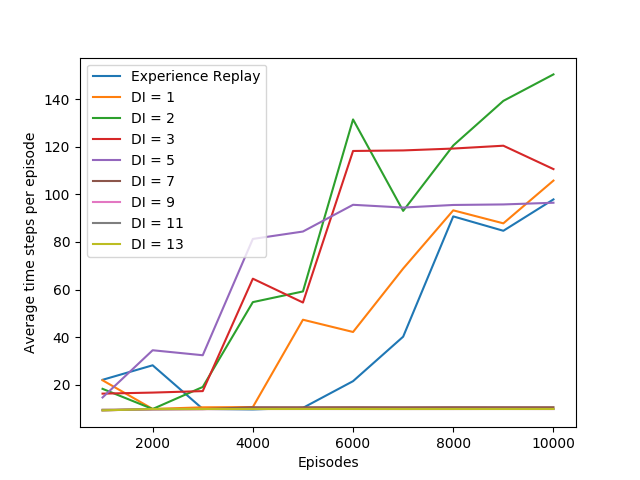
\includegraphics[scale=0.75]{ExpReplay_cartPole.png}
  \caption{DI Experience Replay on CartPole}
  \label{fig:expReplay}
\end{figure}

\subsection{DI REINFORCE}
Refer to Figure \ref{fig:rein} for the plot
\begin{figure}
    
  \centering
  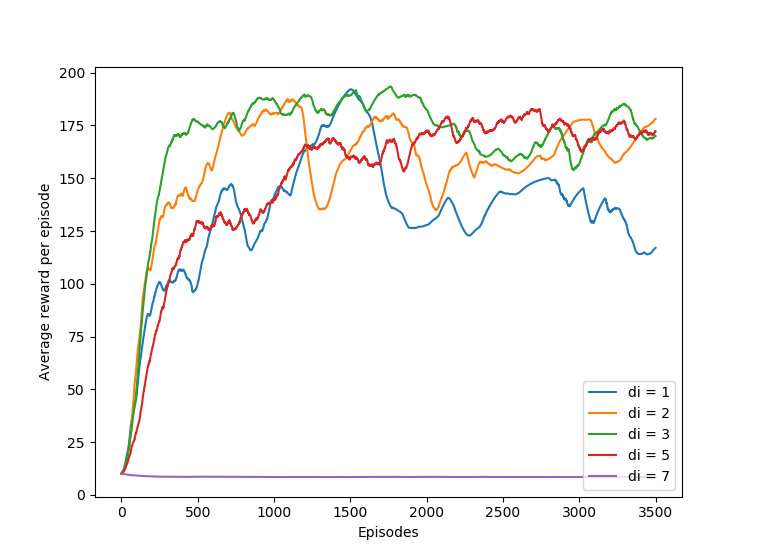
\includegraphics[scale=0.7]{Reinforce_CartPole.png}
  \caption{DI Reinforce on CartPole}
\label{fig:rein}
\end{figure}

\subsection{DI Q-Learning}
MountainCar which is a relatively simple task compared to CartPole shows interesting trends as can be seen in Figure \ref{fig:qmountain}. The vanilla Q-learning tops out with a mean reward of around -130 after 10000 iterations. Large DI like d=7,10 are slightly better than this, but with small d=2,3,5 we able to achieve -118 as the mean reward. A surprising result is obtained with d=30 when the agent learns to get mean reward of -105. The hyposthesis that larger DI will always give better mean is refuted by d=55 where the agent is not able to learn much.\\
A possible explanation for the observations is that with smaller values of d the agent benefits because the updates are made faster and more accurately for every dth state. In this task the state space is actually quite simple. A simple human strategy would be to accelerate to right till a certain point, then accelerate to the left till a large height, and then go right using the force of gravity to your advantage. Thus there is no requirement for the policy to be different with respect to neighbouring states. \\
Following the same action for d steps thus benefits the agent. A steeply large reward for d=30 could be because the number of states till an alternate action is to be chosen is a multiple of the value of d chosen, or that the actual distance moved between states is not very large. In general we want to choose a suitable decision interval which is not too large otherwise we risk the agent not learning anything at all
    
\begin{figure}
    
  \centering
  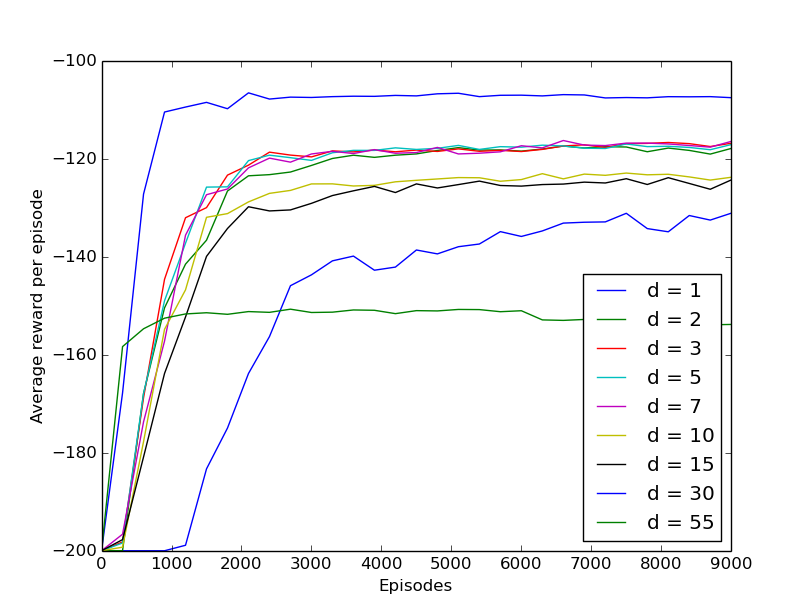
\includegraphics[scale=0.6]{Qlearning_MountainCar.png}
  \caption{DI Q-Learning on MountainCar}
\label{fig:qmountain}
\end{figure}

\section{Conclusion and Future Work}

In this project we establish empirically that in general slowing down of batch reinforcement learning algorithms, Q-learning and policy gradient algorithms seems to improve the performance of the agent. This idea thrives on the underlying fact that in real MDPs we do not need to responsive with respect to each transition, and also propagating less noise in successie updates.\\ Additionally, they take lesser time to execute especially if the update step is computationally expensive, which happens with a frequency inversely proportional to the decision interval.

\section{Future Work}
We experimentally showed the superior performance of slowed-down RL metohds, but do not give any theoretical backing for it. That could be a good path for further research in this topic. We have only looked at agents which keep a fixed value for DI throughout the course of learning. It could be possible that changing it during the run, somewhere on the lines of decaying learning rate and other parameters could further improve performance.  

\bibliography{references}
\bibliographystyle{unsrtnat}


\end{document}
